\documentclass[9pt,t]{beamer}
\usetheme{Wisconsin}
\usepackage[utf8]{inputenc}
\setbeamertemplate{page number in head/foot}[totalframenumber]
\setbeamerfont{title}{size=\LARGE}
\setbeamerfont{subtitle}{size=\Large}
\setbeamerfont{block body}{size=\footnotesize}
\setbeamerfont{author}{size=\LARGE}
\setbeamerfont{date}{size=\Large}
\setlength{\leftmargini}{0pt}

%subcaptions
\usepackage{subcaption}
% \captionsetup[subfigure]{labelformat=empty} % turn off labeling figures

% turn off Figure in captions
\usepackage{caption}
% \captionsetup[figure]{labelformat=empty}

\newcommand{\QOR}{\qquad \text{OR} \qquad}
\newcommand{\QAND}{\qquad \text{AND} \qquad}
\newcommand{\QTHUS}{\qquad \text{THUS} \qquad}
\newcommand{\QTHEN}{\qquad \text{THEN} \qquad}
\newcommand{\QWITH}{\qquad \text{WITH} \qquad}
\newcommand{\QFOR}{\qquad \text{FOR} \qquad}
\newcommand{\QSO}{\qquad \text{SO} \qquad}
\newcommand{\QWHERE}{\qquad \text{WHERE} \qquad}
\newcommand{\LINE}{\par\noindent\rule{\textwidth}{0.4pt}\par}
\newcommand{\toinf}{\rightarrow\infty}
\newcommand{\tozero}{\rightarrow0}
\newcommand{\qeq}{\overset{?}{=}}
\newcommand{\ceq}{\overset{\checkmark}{=}}
\renewcommand{\epsilon}{\varepsilon}
\newcommand{\keff}{$k_{e\!f\!f}$}


% table packages
\usepackage{booktabs}

% Roman Numerals
\newcommand{\rom}[1]{\expandafter\uppercase{\Romannumeral #1\relax}}

% hypersetup
\usepackage{hyperref}
\hypersetup{colorlinks,
            linkcolor = white,
            citecolor = white,
            urlcolor = cyan
}


\def\brac#1{\{#1\}}
\def\Brac#1{\big\{#1\big\}}
\def\BRAC#1{\bigg\{#1\bigg\}}
\def\angbrac#1{\langle#1\rangle}
\def\Angbrac#1{\big\langle#1\big\rangle}
\def\ANGBRAC#1{\bigg\langle#1\bigg\rangle}

% % Transitional slides between sections
% \AtBeginSection[]
% {
%     \begin{frame}
%         \frametitle{Table of Contents}
%         \tableofcontents[currentsection]
%     \end{frame}
% }


% Bibliography
\usepackage[sorting=none]{biblatex} %Imports biblatex package and cites in order of appearance
\addbibresource{mc2023_pres.bib} %Import the bibliography file
% make all font colors white
\setbeamercolor{bibliography item}{fg=white}
\setbeamercolor{bibliography entry author}{fg=white}
\setbeamercolor{bibliography entry title}{fg=white}
\setbeamercolor{bibliography entry location}{fg=white}
\setbeamercolor{bibliography entry note}{fg=white}
% adds numeric labels linked to bib entries
\setbeamertemplate{bibliography item}{\insertbiblabel}

% eliminate header within an environment
\makeatletter
    \newenvironment{withoutheadline}{
       \setbeamertemplate{headline}[default]
       \def\beamer@entrycode{\vspace*{-\headheight}}
    }{}
\makeatother

% appendix renumbering
\usepackage{appendixnumberbeamer}
% frame breaks with same title
\setbeamertemplate{frametitle continuation}[from second][]

\title{Verification of the Cardinal Multiphysics Solver}
\subtitle{1-D Coupled Heat Transfer and Neutron Transport}
\author{Lewis Gross, April Novak, Patrick Shriwise, and Paul Wilson\vspace*{-1cm}}
\date{August 15, 2022}
%%----------------------------------------------------------------------------%%
\begin{document}

\begin{withoutheadline}
\begin{frame}[plain] % the plain makes the first frame look good
    \maketitle
\end{frame}
\end{withoutheadline}

%%----------------------------------------------------------------------------%%
%% Overview
%%----------------------------------------------------------------------------%%
\begin{withoutheadline}
\begin{frame}{Outline}
  \tableofcontents
\end{frame}
\end{withoutheadline}


%%----------------------------------------------------------------------------%%
%% Section 1
%%----------------------------------------------------------------------------%%
\section{Introduction}
\begin{frame}{Modern Multiphysics Simulation and the Importance of V\&V}
    \begin{figure}[H]
        \centering
        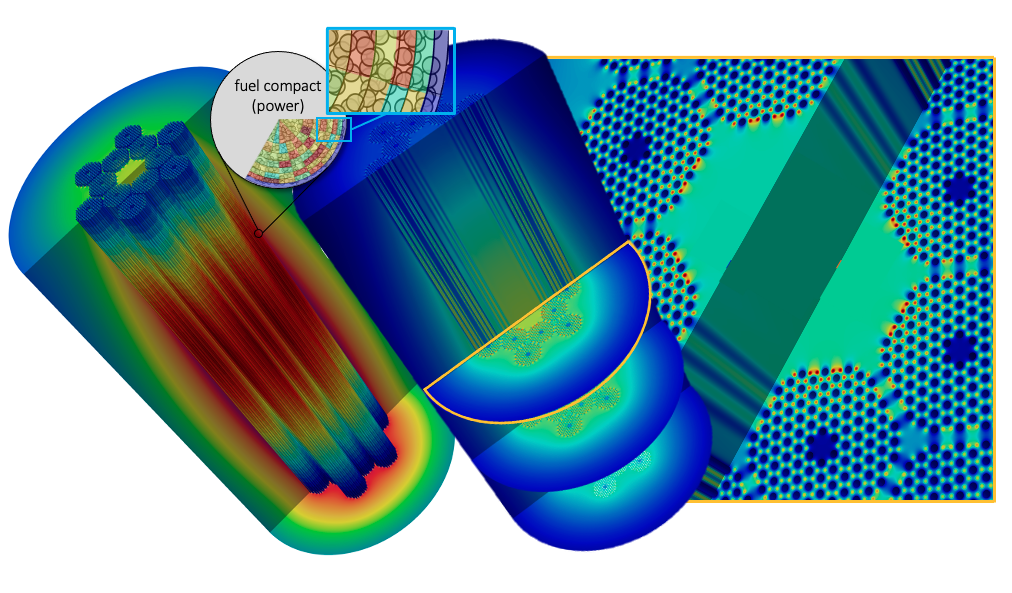
\includegraphics[width=0.875\linewidth]{figures/assembly_solid_temp_fine.png}
    \end{figure}
    \begin{itemize}
        \item Full-core multiphysics model of an HTGR using Cardinal: OpenMC power (left) and MOOSE solid temperature (right) \cite{novak2022-cardinal}.
    \end{itemize}
\end{frame}

\begin{frame}{Modern Multiphysics Simulation and the Importance of V\&V}
    \pause
    \begin{itemize}
        % \item High Fidelity multiphysics simulations are the future of reactor design.
        \item <2-> Many new emerging tools have great potential, but they require Verification and Validation (V\&V).
        \item <3-> Verification via analytical benchmarks allow measurement of true error for a numerical simulation.
        \item <4-> Greisheimer and Kooreman presented a 1-D analytical benchmark that features coupled heat transfer and neutron transport \cite{analytical-benchmark}.
        \item <5-> Cardinal \cite{novak2022-cardinal} our software choice to model this benchmark couples OpenMC \cite{openmc} neutronics and NekRS \cite{nekrs} CFD into the MOOSE framework \cite{lindsay2022moose}.
    \end{itemize}
\end{frame}

\begin{frame}{Cardinal's connection to the MOOSE Framework \cite{cardinal-tutorials}}
    \begin{figure}[H]
        \centering
        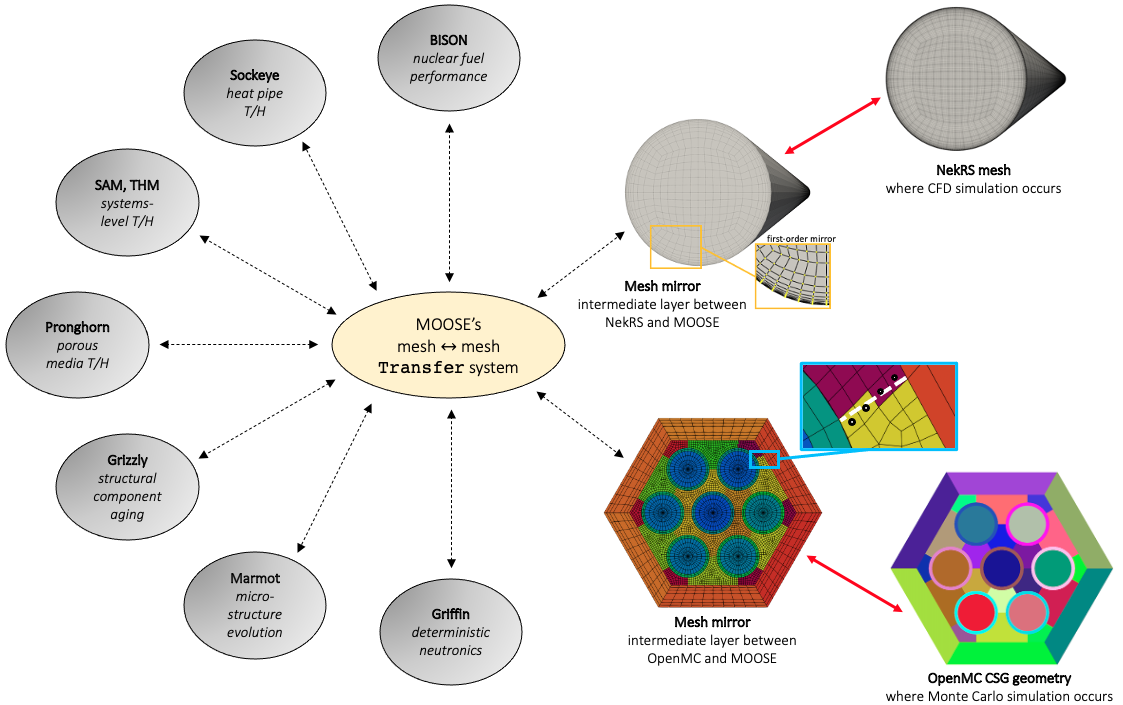
\includegraphics[width=0.9\linewidth]{figures/framework.png}
    \end{figure}
\end{frame}


%%----------------------------------------------------------------------------%%
%% Section 2
%%----------------------------------------------------------------------------%%
\section{Analytical Benchmark}
\begin{frame}{Analytical Benchmark}
    \pause
    \begin{itemize}
        \item <2-> This analytical benchmark includes
        \begin{itemize}
            \item <3-> $S_{2}$ transport: particles restricted to the $\pm$x direction.
            \item <4-> Doppler-broadening
            \begin{equation}\label{doppler-micro-xs}
                \sigma_{t}(x) = \sigma_{t,0}\sqrt{\frac{T_{0}}{T(x)}}
            \end{equation}
            \item <5-> 1-D thermal expansion
            \begin{equation} \label{density-temp-relation}
                \rho(x) =  \rho_{0} \sqrt{\frac{T_{0}}{T(x)}}
            \end{equation}
            \item <6-> Linear temperature dependence for thermal conductivity
            \begin{equation}\label{thermal-conductivity-temp-relation}
                \kappa(x) = \kappa_{0} T(x)
            \end{equation}
        \end{itemize}\vspace*{-0.4cm}
        \item <7->  Using (\ref{doppler-micro-xs}) and (\ref{density-temp-relation}) gives a Doppler-broadened, macroscopic, total cross section that accounts for changes in density due to temperature as
        \begin{equation}
            \Sigma_{t}(x) = \frac{\rho_{0}\sigma_{t,0} N_{A}}{A} \frac{T_{0}}{T(x)}
            \equiv\Sigma_{t,0}\frac{T_{0}}{T(x)}
        \end{equation}
        \item <7-> where $ \sigma_{t,0}$ is the total microscopic cross section at $T_{0}$, $N_{A}$ is Avogadro's number, and $A$ is the mass number
        of the medium.
        \end{itemize}
\end{frame}

\begin{frame}{Analytical Benchmark}
    \begin{itemize}
        \item <1-> Based on 1-D $S_{2}$ transport, the neutron flux $\phi(x)$ is governed by
        \begin{equation}
            \frac{d}{dx}\left\lbrack\frac{1}{\Sigma_{t}(x)} \frac{d\phi(x)}{dx} \right\rbrack + \Sigma_{t}(x)
            \left(\lambda - 1\right)\phi(x) = 0
        \end{equation}
        \item <1-> where $\lambda \equiv (\frac{1}{k_{eff}}\frac{\nu \Sigma_{f}}{\Sigma_{t}} + \frac{\Sigma_{s}}{\Sigma_{t}} )$ is the combined in-scattering and quasi-static fission source term \cite{analytical-benchmark}.
        \item <2->  The conduction equation and its boundary condition govern energy conservation in the slab:
        \begin{multline}
            \frac{d}{dx}\left\lbrack\kappa(T)\frac{dT(x)}{dx}\right\rbrack + q \Sigma_{t}(x)\phi(x) = 0
            \QAND \\
            - \kappa(T) \frac{dT}{dx} \bigg|_{\pm \frac{L}{2}} + h\left[ T(\pm \frac{L}{2}) - T_{0}\right]
        \end{multline}
        \item <2-> where $\kappa$ is the thermal conductivity, $q$ is the energy released \textbf{per reaction}, $\Sigma_{t}$ is the total macroscopic cross section, and $h$ is the heat transfer coefficient.
    \end{itemize}
\end{frame}


\begin{frame}{System Domain, Differential Equations, and Boundary Conditions}
    \begin{figure}[T]
        \centering
        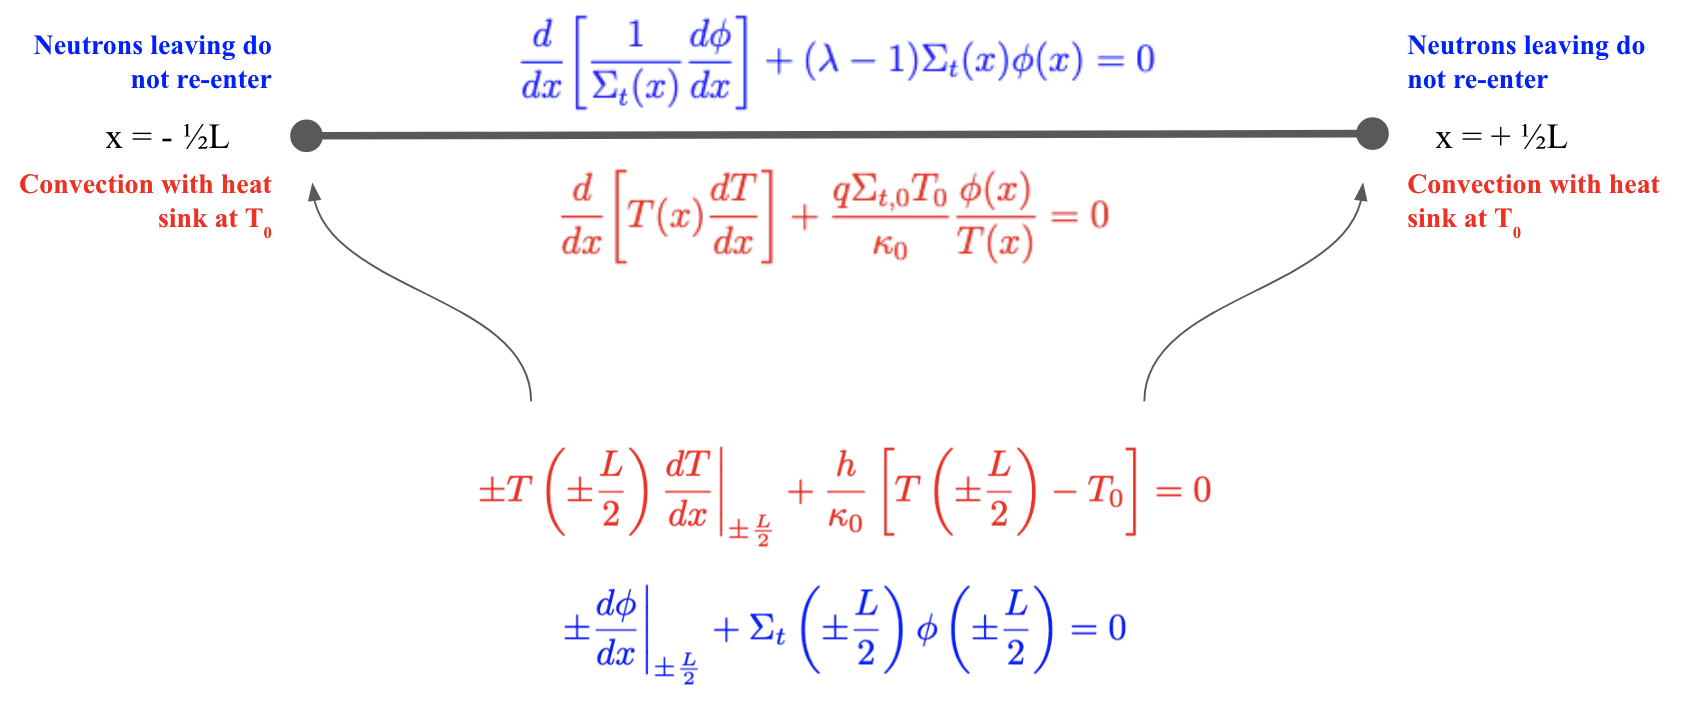
\includegraphics[width=0.725\linewidth]{figures/1D_Benchmark_Diagram.png}<1->
    \end{figure}
    \begin{itemize}
        \item <2-> The fundamental assumption (ansatz) of \cite{analytical-benchmark}: $T(x)=f\phi(x)$.
        \item <3-> This imposes two constraints that determine the system heat transfer coefficient $h$ and the
        total microscopic cross section $\sigma_{t,0}$. The solution that satisfies the above is given by
        an elliptical flux shape
        \begin{equation}
            \phi(x) = \phi(0) \sqrt{1 - \frac{(\lambda - 1)P^{2}x^{2}}{L^{2}q^{2}\phi^2(0)}}
        \end{equation}
        \item <3-> where $P$ is the slab power and $L$ is the slab equilibrium length.
    \end{itemize}
\end{frame}

%%----------------------------------------------------------------------------%%
%% Section 3
%%----------------------------------------------------------------------------%%
\section{Computational Model}
\begin{frame}{OpenMC Model}
    \pause
    \begin{itemize}
        \item <2-> Slab geometry divided into N cells, $N=[5, 10, 25, 50, 100, 250, 500, 1000]$.
        \item <3-> Equilibrium length $L=106.47$ cm in the x-direction, $1$ cm in the y-direction, $1$ cm in the z-direction.
        \begin{itemize}
            \item <4-> Internal X-planes use transmissive BCs and boundary X-planes use vacuum BCs.
            \item <5-> Y and Z-planes reflective BCs to simulate infiniteness.
        \end{itemize}
        \item <6-> Macroscopic XS library via OpenMC's \texttt{XSData} class. It uses the macroscopic XS to account for changes in the XS due to temperature-density feedback on the equilibrium mesh instead of modeling thermal expansion via mesh deformation.
        \item <7-> Mesh deformation is possible in Cardinal via DAGMC \cite{novak-2023}.
        \item <8-> XS library has data for every integer temperature between 308 K and 358 K and rounds to nearest for a lookup between two data points.
        \item <9-> XS library uses one energy group from $0$ to $20$ MeV.
        \item <10-> $S_{2}$ patch to restrict particle birth direction and scattering direction to only $\pm$x.
        \item <11->Tallies flux, kappa-fission heating rate, and $k$-eigenvalue.
    \end{itemize}
\end{frame}

\begin{frame}{MOOSE Heat Conduction Model}
    \pause
    \begin{itemize}
        \item <2-> Mesh with identical dimensions as OpenMC model. Allows 1:1 feedback between single physics solves.
        \item <3-> MOOSE accepts heating rate in each mesh element from OpenMC and solves for temperature distribution.
        \item <4-> Convective boundary conditions at end points with heat sink at $T_{0}=293$ K.
        \item <5-> Jacobi Free Newton Krylov solver: $10^{-7}$ absolute tolerance and $10^{-9}$ relative tolerance.
    \end{itemize}
\end{frame}

\begin{frame}{Coupling, Data Mapping \cite{cardinal-tutorials}, and Convergence Criteria}
    \pause
    \begin{figure}[T]
        \centering
        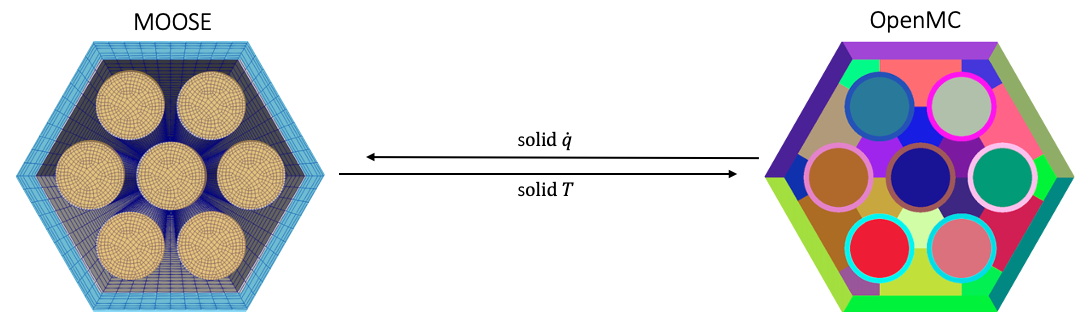
\includegraphics[width=\linewidth]{figures/cardinal_solid.png}<2->
    \end{figure}
    \begin{itemize}
        \item <3-> 200 Picard Iterations.  Did not use steady state detection, though MOOSE has this capability. Robbins-Monro relaxation assisted tally statistics \cite{dufek}.
        \item <4-> $k$-eigenvalue simulation used 50,000 particles per batch, 50 inactive batches and 100 active batches.
        \begin{itemize}
            \item <5-> Shannon Entropy study confirmed this sufficient following criteria from \cite{brown-entropy-2006}.
        \end{itemize}
        \item <6-> Final transport solve with converged temperature used 250,000 particles per batch.
    \end{itemize}
\end{frame}


%%----------------------------------------------------------------------------%%
%% Section 4
%%----------------------------------------------------------------------------%%
\section{Results and Discussion}
\begin{frame}{Outputs and Comparisons}
    \begin{figure}[T]
        \hspace*{-1cm}
        \begin{subfigure}[b]{0.495\linewidth}
            \centering
            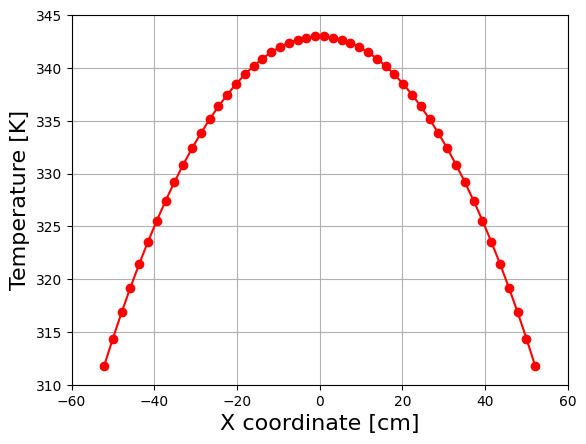
\includegraphics[height=0.85\linewidth]{figures/temp_50.png}
        \end{subfigure}\hspace*{0.6cm}
        \begin{subfigure}[b]{0.495\linewidth}
        \centering
            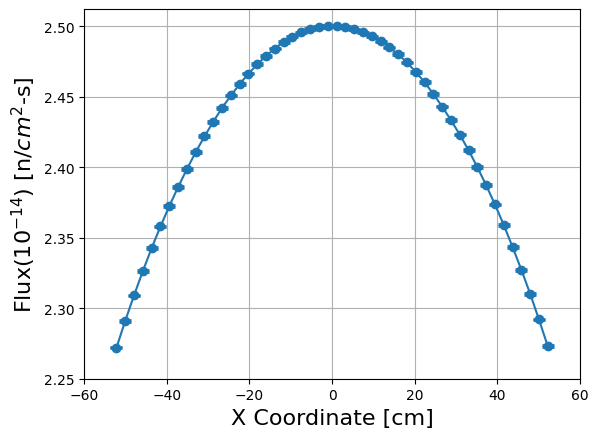
\includegraphics[height=0.85\linewidth]{figures/flux_50.png}
        \end{subfigure}
    \end{figure}
    \begin{itemize}
        \item Numerical solutions for 50 mesh elements. On the right, error bars show the relative error of the flux, which are nearly smaller than the circular marker sizes.
    \end{itemize}
\end{frame}

\begin{frame}{Solution $L_{2}$ Error Norms}
    \begin{figure}[T]
        \hspace*{-0.9cm}
        \begin{subfigure}{0.4995\linewidth}
            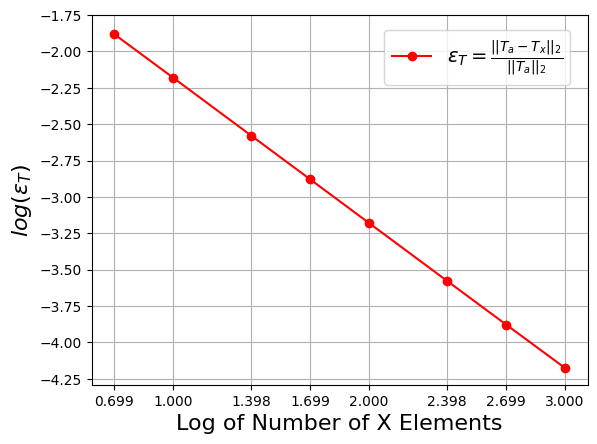
\includegraphics[height=0.85\linewidth]{figures/temp_error_norms.png}
        \end{subfigure}\hspace*{0.85cm}
        \begin{subfigure}{0.4995\linewidth}
            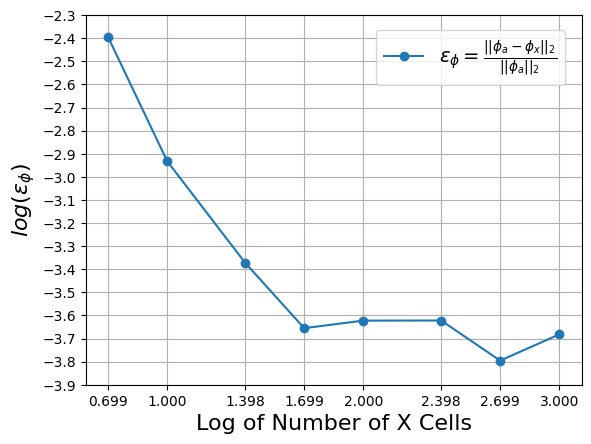
\includegraphics[height=0.85\linewidth]{figures/flux_error_norms.png}
        \end{subfigure}
    \end{figure}
    \begin{itemize}
        \item Error norms as a function of heat conduction mesh element count and OpenMC cell count, respectively.
    \end{itemize}
\end{frame}

\begin{frame}{Eigenvalue comparisons across each spatial discretization}
    \begin{table}[H]
        \centering
        \begin{tabular}{@{}ccc@{}}
            \toprule
            Resolution &  \keff & (numerical - analytical) [pcm]\\
            \midrule
            analytical & 0.29557 & - \\
            \midrule
            5    & 0.29624 $\pm$ 0.00003 & \phantom{-}67 $\pm$ 3 \\
            10   & 0.29581 $\pm$ 0.00004 & \phantom{-}24 $\pm$ 4 \\
            25   & 0.29563 $\pm$ 0.00004 & \phantom{-}6  $\pm$ 4 \\
            50   & 0.29553 $\pm$ 0.00004 &           -4  $\pm$ 4 \\
            100  & 0.29557 $\pm$ 0.00003 & \phantom{-}0  $\pm$ 3 \\
            250  & 0.29561 $\pm$ 0.00004 & \phantom{-}4  $\pm$ 4 \\
            500  & 0.29561 $\pm$ 0.00004 & \phantom{-}4  $\pm$ 4 \\
            1000 & 0.29558 $\pm$ 0.00004 & \phantom{-}1  $\pm$ 4 \\
        \bottomrule
        \end{tabular}
    \end{table}
    \begin{itemize}
        \item<2-> \keff is a system-wide parameter, so it converges much faster than flux and is not as dependent on number of cells.
    \end{itemize}
\end{frame}

\begin{frame}{Computed to Expected Ratios}
    \vspace*{-0.4cm}
    \begin{figure}[T]
        \hspace*{-0.87cm}
        \begin{subfigure}{0.495\linewidth}
            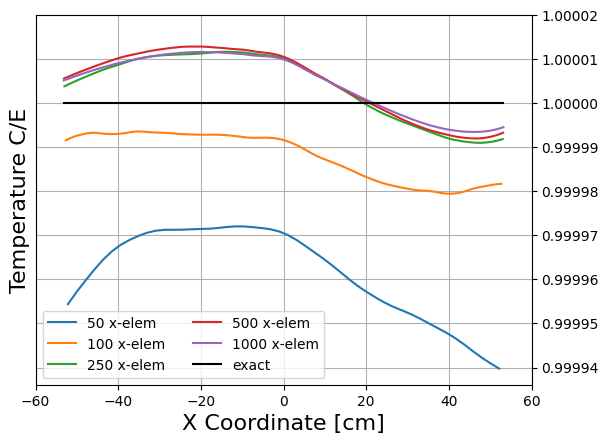
\includegraphics[height=0.85\linewidth]{figures/fine_temp_num_to_analy_ratios.png}
        \end{subfigure}\hspace*{0.85cm}
        \begin{subfigure}{0.495\linewidth}
            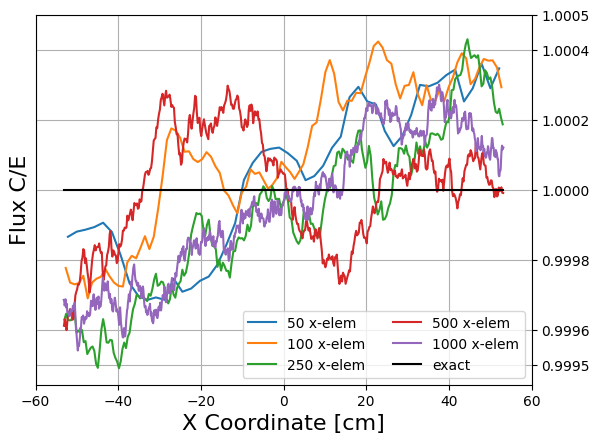
\includegraphics[height=0.85\linewidth]{figures/fine_flux_num_to_analy_ratios.png}
        \end{subfigure}
    \end{figure}
    \begin{itemize}
        \item $C/E$ for fine cases ($N=50,100,250,500,1000$). Note the scales of the $y$-axes - the temperature is everywhere being predicted to within 0.006\% and flux is everywhere being predicted to within 0.05\%.
    \end{itemize}
\end{frame}

\begin{frame}{Individual Flux $C/E$ with $2\sigma$ Error Bars for Fine Cases}
    \begin{figure}[T]
        \hspace*{-1.1cm}
        \begin{subfigure}{0.495\textwidth}
            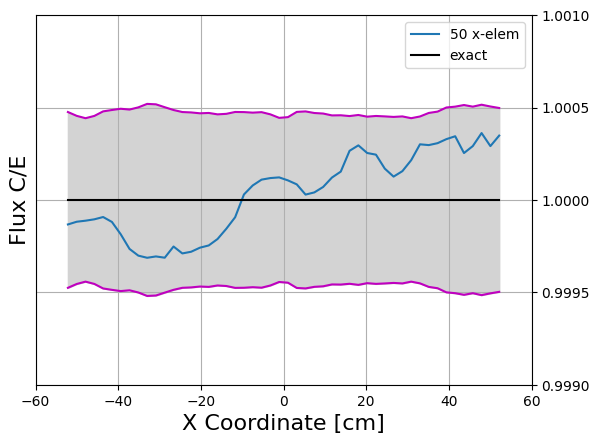
\includegraphics[width=1.18\linewidth]{figures/50_flux_CE_error_bars.png}
        \end{subfigure}\hspace*{0.89cm}
        \begin{subfigure}{0.495\textwidth}
            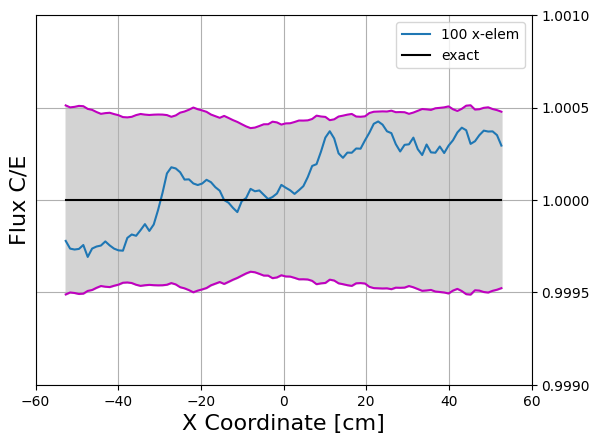
\includegraphics[width=1.18\linewidth]{figures/100_flux_CE_error_bars.png}
        \end{subfigure}
    \end{figure}
    \begin{itemize}
        \item $C/E$ in blue with $2\sigma$ error bars (gray bounded by purple). $50$ and $100$ cells.
    \end{itemize}
\end{frame}

\begin{frame}{Individual Flux $C/E$ with $2\sigma$ Error Bars for Fine Cases}
    \begin{figure}[T]
        \hspace*{-1.1cm}
        \begin{subfigure}{0.495\textwidth}
            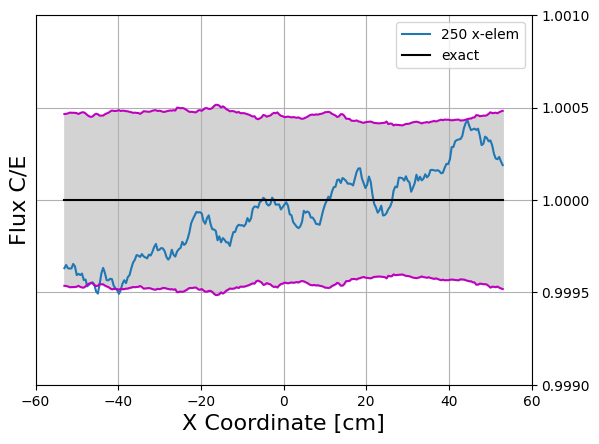
\includegraphics[width=1.18\linewidth]{figures/250_flux_CE_error_bars}
        \end{subfigure}\hspace*{0.89cm}
        \begin{subfigure}{0.495\textwidth}
            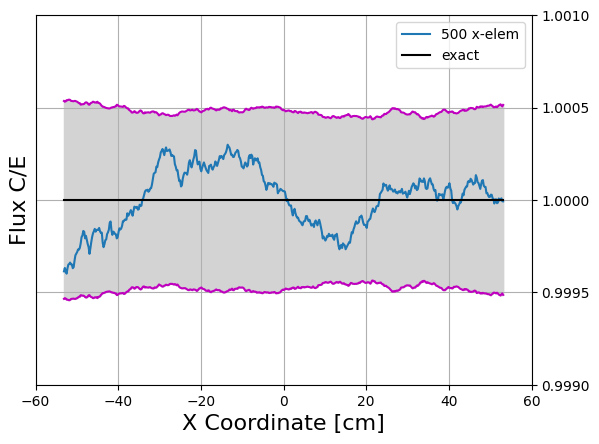
\includegraphics[width=1.18\linewidth]{figures/500_flux_CE_error_bars}
        \end{subfigure}
    \end{figure}
    \begin{itemize}
        \item $C/E$ in blue with $2\sigma$ error bars (gray bounded by purple). $250$ and $500$ cells
    \end{itemize}
\end{frame}

\begin{frame}{Individual Flux $C/E$ with $2\sigma$ Error Bars for Fine Cases}
    \begin{figure}[T]
        \centering
        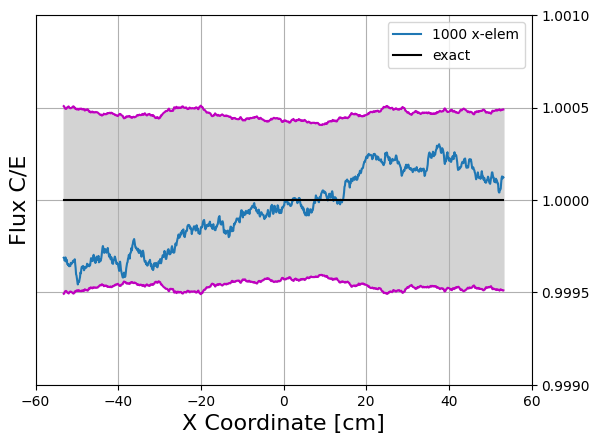
\includegraphics[width=0.7\linewidth]{figures/1000_flux_CE_error_bars}
    \end{figure}
    \begin{itemize}
        \item $C/E$ in blue with $2\sigma$ error bars (gray bounded by purple). $1000$ cells.
    \end{itemize}
\end{frame}

\begin{frame}
\frametitle{Why do the error bars appear on the same order despite cell refinement?}
    \pause
    \begin{figure}[T]
        \centering
        \begin{subfigure}{0.32\textwidth}
            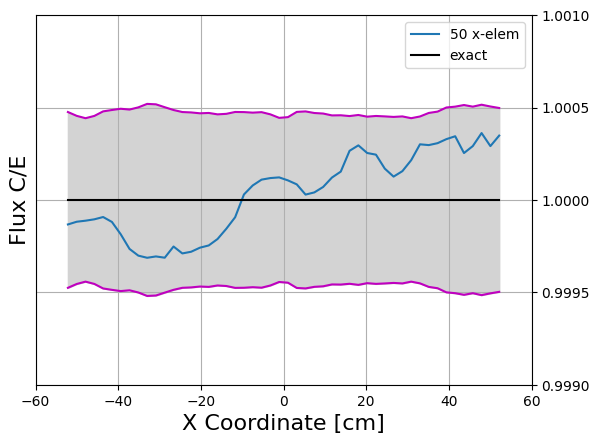
\includegraphics[width=\linewidth]{figures/50_flux_CE_error_bars.png}
        \end{subfigure}
        \begin{subfigure}{0.32\textwidth}
            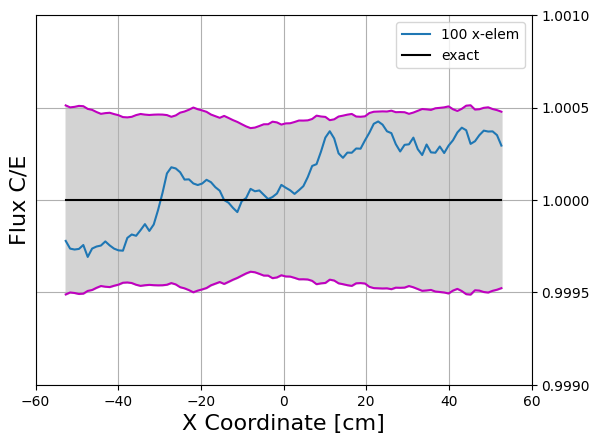
\includegraphics[width=\linewidth]{figures/100_flux_CE_error_bars.png}
        \end{subfigure}
        \begin{subfigure}{0.32\textwidth}
            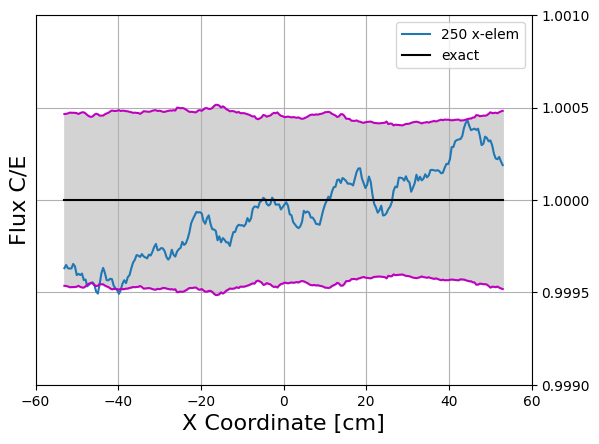
\includegraphics[width=\linewidth]{figures/250_flux_CE_error_bars}
        \end{subfigure}
        \begin{subfigure}{0.32\textwidth}
            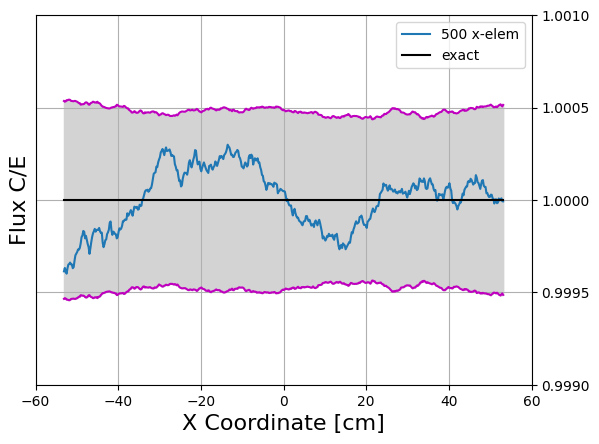
\includegraphics[width=\linewidth]{figures/500_flux_CE_error_bars}
        \end{subfigure}
        \begin{subfigure}{0.32\textwidth}
            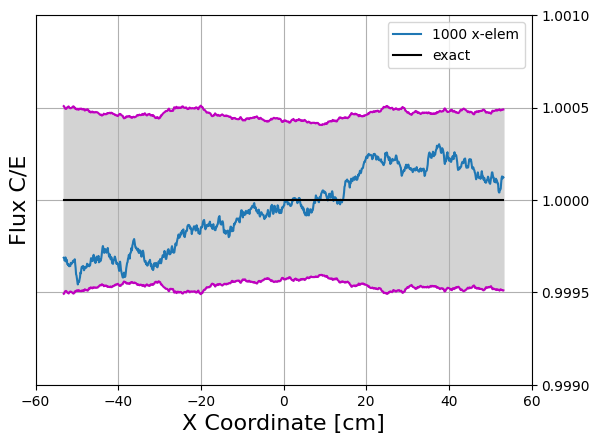
\includegraphics[width=\linewidth]{figures/1000_flux_CE_error_bars}
        \end{subfigure}
    \end{figure}
    \begin{itemize}
        \item <3-> MFP $\in[239,278]$ cm ($L=106.47$ cm). Spatially uniform birth distribution.
        \item <4-> Nearly all points fall within $2\sigma$ (95\% Confidence Interval), meaning that Cardinal is computing the correct flux within statistical uncertainty.
    \end{itemize}
\end{frame}

%%----------------------------------------------------------------------------%%
%% Bibliography
%%----------------------------------------------------------------------------%%

\begin{withoutheadline}
    \begin{frame}{Acknowledgements}
        \begin{itemize}
            \item Benchmark authors: David P. Greisheimer and Gabriel Kooreman
            \item Co-authors: April J. Novak, Patrick Shriwise, Paul P.H. Wilson
            \item OpenMC, Cardinal, and MOOSE teams!
        \end{itemize}
        \begin{figure}[H]
            \centering
            
\includegraphics[width=0.75\linewidth]{figures/openmc_logo.png}
        \end{figure}
        \begin{figure}[H]
            \centering
            
\includegraphics[width=0.75\linewidth]{figures/cardinal_logo.png}
        \end{figure}
        \begin{figure}[H]
            \centering
            
\includegraphics[width=0.75\linewidth]{figures/moose_logo.png}
        \end{figure}
    \end{frame}
\end{withoutheadline}

\begin{withoutheadline}
\begin{frame}[allowframebreaks]{Bibliography}
    \printbibliography
\end{frame}
\end{withoutheadline}

\appendix


\begin{frame}{Coarse $C/E$ results}
    \begin{figure}[T]
        \begin{subfigure}{0.475\linewidth}
            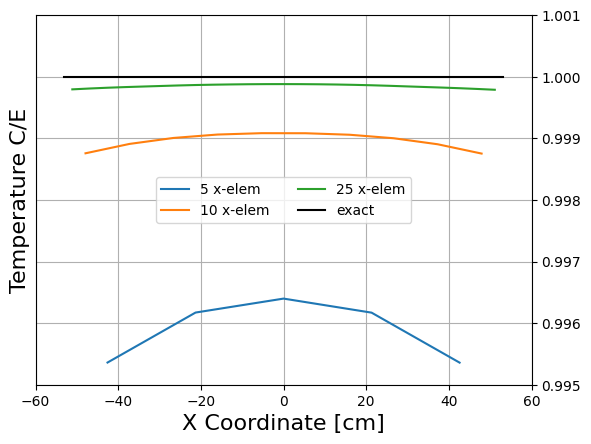
\includegraphics[height=0.8\linewidth]{figures/coarse_temp_num_to_analy_ratios.png}
        \end{subfigure}\hspace{0.3cm}
        \begin{subfigure}{0.475\linewidth}
            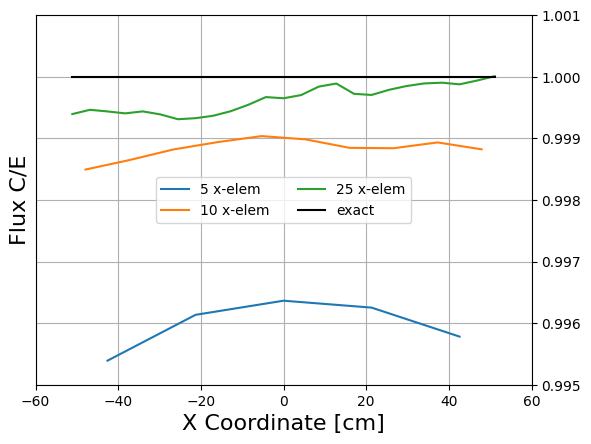
\includegraphics[height=0.8\linewidth]{figures/coarse_flux_num_to_analy_ratios.png}
        \end{subfigure}
    \end{figure}
    \begin{itemize}
        \item $C/E$ for coarse cases ($N=5,10,25$). The coarse cases' errors are a few orders of magnitude larger than the fine cases. A significant improvement in agreement can be seen between each coarse case.
    \end{itemize}
\end{frame}


\begin{withoutheadline}
\begin{frame}[allowframebreaks]{Ensuring Validity of the Fundamental Ansatz}
    \begin{itemize}
        \item Taking the heat conduction ODE
        \begin{equation}
            \frac{d}{dx}\left\lbrack\kappa(T(x))\frac{dT(x)}{dx}\right\rbrack + q \Sigma_{t}(x)\phi(x) = 0
        \end{equation}
        \item and using the thermal conductivity and cross section temperature dependence
        \begin{equation}
            \frac{d}{dx}\left\lbrack\kappa_{0} T(x)\frac{dT(x)}{dx}\right\rbrack + q\Sigma_{t,0}\frac{T_{0}}{T(x)}\phi(x) = 0
        \end{equation}
        \item Taking the neutron transport ODE
        \begin{equation}
            \frac{d}{dx}\left\lbrack\frac{1}{\Sigma_{t}(x)} \frac{d\phi(x)}{dx} \right\rbrack + \Sigma_{t}(x)
            \left(\lambda - 1\right)\phi(x) = 0
        \end{equation}
        \item and inserting cross section temperature dependence gives
        \begin{equation}
            \frac{d}{dx}\left\lbrack  \frac{T(x)}{\Sigma_{t,0}T_{0}} \frac{d\phi(x)}{dx} \right\rbrack + \Sigma_{t,0}\frac{T_{0}}{T(x)}
            \left(\lambda - 1\right)\phi(x) = 0
        \end{equation}
        \item these two equations are very close, and after some re-arranging, they look even closer
        \begin{multline}
            \frac{d}{dx}\left\lbrack T(x)\frac{dT(x)}{dx}\right\rbrack + \frac{q\Sigma_{t,0}}{\kappa_{0}}\frac{T_{0}}{T(x)}\phi(x) = 0
            \QAND \\
            \frac{d}{dx}\left\lbrack  \frac{T(x)}{\Sigma_{t,0}T_{0}} \frac{d\phi(x)}{dx} \right\rbrack + \Sigma_{t,0}\frac{T_{0}}{T(x)}
            \left(\lambda - 1\right)\phi(x) = 0
        \end{multline}
        \item Applying the ansatz $T(x) = f\phi(x)$ gives
        \begin{multline}
            \frac{d}{dx}\left\lbrack f^2\phi(x)\frac{d\phi(x)}{dx}\right\rbrack + \frac{q\Sigma_{t,0}}{\kappa_{0}}\frac{T_{0}}{f} = 0
            \QAND \\
            \frac{d}{dx}\left\lbrack  \frac{f\phi(x)}{\Sigma_{t,0}T_{0}} \frac{d\phi(x)}{dx} \right\rbrack + \Sigma_{t,0}\frac{T_{0}}{f}
            \left(\lambda - 1\right) = 0
        \end{multline}\vspace{-0.5cm}
        \begin{multline}
            \frac{d}{dx}\left\lbrack \phi(x)\frac{d\phi(x)}{dx}\right\rbrack + \frac{q\Sigma_{t,0}}{\kappa_{0}}\frac{T_{0}}{f^3} = 0
            \QAND \\
            \frac{d}{dx}\left\lbrack \phi(x)\frac{d\phi(x)}{dx} \right\rbrack +
            \left(\Sigma_{t,0}\frac{T_{0}}{f}\right)^2 \left(\lambda - 1\right) = 0
        \end{multline}
        \item In order to make the ansatz hold, this implies that
        \begin{equation}
            \frac{q\Sigma_{t,0}}{\kappa_{0}}\frac{T_{0}}{f^3} = \left(\Sigma_{t,0}\frac{T_{0}}{f}\right)^2 \left(\lambda - 1\right)
            \QOR \Sigma_{t,0} = \frac{q}{(\lambda-1)\kappa_{0} T_{0}f}
        \end{equation}
        which is a condition for the total cross section based on system parameters.
        \item A similar process of matching coefficients
        must be applied to the boundary conditions to gain a condition for the heat transfer coefficient. Though, at this point, realize that
        \begin{equation}
            \frac{d}{dx}\left\lbrack \phi(x)\frac{d\phi(x)}{dx} \right\rbrack +
            \left(\Sigma_{t,0}\frac{T_{0}}{f}\right)^2 \left(\lambda - 1\right) = 0
        \end{equation}
        \item is a separable ODE that can be solved for an analytical solution. The result for the heat transfer coefficient is given by
        \begin{equation}
            h \left(\sqrt{\frac{L(\lambda-1)}{\kappa_{0}P}} - \frac{2T_{0}}{P} \right) = 1
        \end{equation}
    \end{itemize}
\end{frame}
\end{withoutheadline}


\begin{withoutheadline}
\begin{frame}[allowframebreaks]{Deriving the Benchmark ODE for $\phi(x)$}
    \begin{itemize}
        \item Going from the steady-state, mono-energetic, 1-D neutron transport equation to the ODE that describes neutron transport for this benchmark:
        \begin{equation}
            \mu \frac{\partial \psi(x,\mu)}{\partial x} + \Sigma_{t}(x)\psi(x,\mu) =
            \int_{-1}^{1} \frac{1}{2}\big[\Sigma_{s}(x) + \frac{\nu \Sigma_{f}(x)}{k_{eff}}\big] \psi(x,\mu')d\mu'
        \end{equation}
        For now, lump the fission term into the scattering cross section to get
        \begin{equation} \label{transport eq}
            \mu \frac{\partial \psi(x,\mu)}{\partial x} + \Sigma_{t}(x)\psi(x,\mu) =
            \int_{-1}^{1} \frac{1}{2}\Sigma_{s}(x) \psi(x,\mu')d\mu'
        \end{equation}
        Define the scalar flux and the magnitude of current
        \begin{equation}
            \phi(x) = \int_{-1}^{1} \psi(x,\mu) d\mu \QAND J(x) = \int_{-1}^{1} \mu \psi(x,\mu) d\mu.
        \end{equation}
        Considering $S_{2}$ transport means restricting the angular cosine to $\mu = \pm 1$:
        \begin{equation}
            \psi(x,\mu) = \psi(x,-1) \delta(\mu+1) + \psi(x,1) \delta(\mu-1)
        \end{equation}
        (sometimes denoted $\psi^{+}\equiv \psi(x,1) \delta(\mu-1) $ and $\psi^{-}\equiv \psi(x,-1) \delta(\mu+1) $)
        \newpage
        Now carrying out the integral definitions with $S_{2}$ quantities gives
        \begin{equation} \label{scalar flux}
            \phi(x) = \int_{-1}^{1} \left\lbrack \psi(x,-1) \delta(\mu+1) + \psi(x,1) \delta(\mu-1) \right\rbrack d\mu =
            \psi(x,-1) + \psi(x,1)
        \end{equation}
        and
        \begin{equation} \label{current}
            J(x) = \int_{-1}^{1} \mu \left\lbrack \psi(x,-1) \delta(\mu+1) + \psi(x,1) \delta(\mu-1) \right\rbrack d\mu =
            \psi(x,1) - \psi(x,-1)
        \end{equation}
        Evaluating (\ref{transport eq}) at $\mu=\pm 1$ gives
        \begin{equation} \label{-1}
            -\frac{\partial \psi(x,-1)}{\partial x} + \Sigma_{t}(x)\psi(x,-1) =
            \frac{1}{2}\Sigma_{s}(x) \phi(x);
        \end{equation}
        \begin{equation} \label{+1}
            \frac{\partial \psi(x,1)}{\partial x} + \Sigma_{t}(x)\psi(x,1) =
            \frac{1}{2}\Sigma_{s}(x) \phi(x).
        \end{equation}
        Adding (\ref{-1}) and (\ref{+1}) gives
        \begin{equation}\label{sum}
            -\frac{\partial \psi(x,-1)}{\partial x} + \frac{\partial \psi(x,1)}{\partial x} + \Sigma_{t}(x)\left(\psi(x,-1) + \psi(x,1) \right) =
            \Sigma_{s}(x) \phi(x)
        \end{equation}
        The results for $\phi(x)$ and $J(x)$ can simplify (\ref{sum})
        \begin{equation}  \label{current derivative}
            \frac{dJ(x)}{ dx} + \Sigma_{t}(x)\phi(x) =
            \Sigma_{s}(x) \phi(x)
        \end{equation}
        Subtracting  (\ref{-1}) and (\ref{+1}) gives
        \begin{equation}
            -\frac{\partial \psi(x,-1)}{dx}
            - \frac{\partial \psi(x,1)}{d x} + \Sigma_{t}(x)\left(\psi(x,-1)  - \Sigma_{t}(x)\psi(x,1)\right) =
            0
        \end{equation}
        Which can be transformed with similar tricks to
        \begin{equation} \label{flux derrivative}
            \frac{d\phi(x)}{dx} + \Sigma_{t}(x)J(x) = 0 \QOR
            J(x) = - \frac{1}{\Sigma_{t}(x)} \frac{d\phi(x)}{dx}
        \end{equation}
        Since $\frac{dJ(x)}{dx}$ appears in (\ref{current derivative}), we can take the derivative of both sides of (\ref{flux derrivative}) and substitute it in
        \begin{equation}
          \frac{dJ(x)}{dx} =
          - \frac{d}{dx} \left\lbrack \frac{1}{\Sigma_{t}(x)} \frac{d\phi(x)}{dx} \right\rbrack
        \end{equation}
        Now the equation that only depends on $\phi(x)$ is given by
        \begin{equation}
            -\frac{d}{dx}\left\lbrack\frac{1}{\Sigma_{t}(x)} \frac{d\phi(x)}{dx} \right\rbrack + \Sigma_{t}(x)\phi(x) =
            \Sigma_{s}(x) \phi(x)
        \end{equation}
        At this point, we ``un-lump" the scattering cross section to write out the fission term
        \begin{equation}
            -\frac{d}{dx}\left\lbrack\frac{1}{\Sigma_{t}(x)} \frac{d\phi(x)}{dx} \right\rbrack + \Sigma_{t}(x)\phi(x) =
            \left\lbrack\Sigma_{s}(x) + \frac{\nu \Sigma_{f}}{k_{eff}}\right\rbrack\phi(x)
        \end{equation}
        \begin{equation}
            -\frac{d}{dx}\left\lbrack\frac{1}{\Sigma_{t}(x)} \frac{d\phi(x)}{dx} \right\rbrack + \Sigma_{t}(x)
            \left\lbrack1 - \frac{\Sigma_{s}(x) + \frac{\nu \Sigma_{f}}{k_{eff}}}{\Sigma_{t}}\right\rbrack\phi(x) = 0
        \end{equation}
        \begin{equation}
            \frac{d}{dx}\left\lbrack\frac{1}{\Sigma_{t}(x)} \frac{d\phi(x)}{dx} \right\rbrack + \Sigma_{t}(x)
            \left\lbrack\frac{\Sigma_{s}(x) + \frac{\nu \Sigma_{f}}{k_{eff}}}{\Sigma_{t}} - 1\right\rbrack\phi(x) = 0
        \end{equation}
        Now define
        \begin{equation}
            \lambda \equiv \frac{\Sigma_{s}(x) + \frac{\nu \Sigma_{f}}{k_{eff}}}{\Sigma_{t}}
        \end{equation}
        giving the final result:
        \begin{equation}
            \frac{d}{dx}\left\lbrack\frac{1}{\Sigma_{t}(x)} \frac{d\phi(x)}{dx} \right\rbrack + \Sigma_{t}(x)
            \left(\lambda - 1\right)\phi(x) = 0
        \end{equation}
        \newpage
        The next task is to apply boundary conditions so that $\phi(x)$ can be specified. In discrete ordinates with $\mu=\pm1$ ($S_{2}$), we use the vacuum boundary condition. The angular flux for positive angular cosines is zero at the left boundary and is zero for negative angular cosines at the right boundary.
        Using the previous results for $\phi(x)$ and $J(x)$ at the boundaries gives
        \begin{multline}
            \phi(x=\frac{L}{2}) =  \psi(x=\frac{L}{2},\mu =-1) + \psi(x=\frac{L}{2},\mu =1) \QAND  \\ \phi(x=-\frac{L}{2}) =  \psi(x=-\frac{L}{2},\mu =-1) + \psi(x=-\frac{L}{2},\mu =1)
        \end{multline}
        and
        \begin{multline}
            J(x=\frac{L}{2}) = - \psi(x=\frac{L}{2},-1)  + \psi(x=\frac{L}{2},1) \QAND \\ J(x=-\frac{L}{2}) = - \psi(x=-\frac{L}{2},-1)  + \psi(x=-\frac{L}{2},1)
        \end{multline}
        Now, terms can be crossed out due to vacuum boundaries. This gives that
        \begin{multline}
            \phi(x=\frac{L}{2}) =  \psi(x=\frac{L}{2},\mu =1) \QAND \\ \phi(x=-\frac{L}{2}) =  \psi(x=-\frac{L}{2},\mu =-1)
        \end{multline}
        \vspace*{-0.4cm}
        \begin{multline}
            J(x=\frac{L}{2}) = \psi(x=\frac{L}{2},\mu =1) \QAND \\ J(x=-\frac{L}{2}) = - \psi(x=-\frac{L}{2},\mu =-1)
        \end{multline}
        Using this with (\ref{flux derrivative}) gives the desired boundary conditions
        \begin{equation}
            J(x=\pm \frac{L}{2}) = \pm \phi(x=\pm \frac{L}{2})
        \end{equation}
        And the boundary conditions of interest are now
        \begin{equation}
            \frac{d\phi}{dx}\bigg|_{x=\pm \frac{L}{2}} \pm  \Sigma_{t}(x=\pm \frac{L}{2})  \phi(x=\pm \frac{L}{2})  = 0
        \end{equation}
    \end{itemize}
\end{frame}
\end{withoutheadline}

\end{document}
